\documentclass[paper=a4, fontsize=9pt]{scrartcl}
\usepackage[bottom=0.9in, left=0.7in, right=0.7in, top=0.8in, foot=0.5in]{geometry}
\usepackage{layouts}

\usepackage[usenames,dvipsnames,x11names]{xcolor}

\usepackage[T1]{fontenc}
\usepackage{fourier}
\usepackage[english]{babel}
\usepackage{amsmath,amsfonts,amsthm}

\usepackage{sectsty}
\allsectionsfont{\centering \normalfont\scshape}

\usepackage{acronym}
\usepackage{booktabs}
\usepackage{caption}
\usepackage{fancyhdr}
\usepackage{float}
\usepackage{graphicx}
\usepackage[htt]{hyphenat}
\usepackage{lastpage}
\usepackage{multicol}
\usepackage{titlesec}
\usepackage[inline]{enumitem}
\usepackage{algorithm, algpseudocode}
\usepackage[export]{adjustbox}
\usepackage{pdflscape}

\usepackage{tikz}
\usepackage{pgfplots, pgfplotstable}
\pgfplotsset{compat=1.5}
\usepgfplotslibrary{colorbrewer}

\pagestyle{fancyplain}
\fancyhead{}
\fancyfoot[L]{}
\fancyfoot[C]{\thepage~of~4}
\renewcommand{\headrulewidth}{0pt}
\renewcommand{\footrulewidth}{0pt}
\setlength{\headheight}{13.6pt}

\newcommand{\horrule}[1]{\rule{\linewidth}{#1}}

\title{
\vspace{-1cm}
\normalfont \normalsize
\textsc{Norwegian University of Science and Technology\\IT3708 -- Bio-Inspired Artificial Intelligence}
\horrule{0.5pt} \\[0cm]
\Huge Project 4: Solving Job Shop Scheduling Problem\\Using Bio-Inspired Algorithms\\[-0.3cm]
\horrule{2pt} \\[0.1cm]
}

\newacro{ACO}{Ant Colony Optimization}
\newacro{BA}{Bees Algorithm}
\newacro{PSO}{Particle Swarm Optimization}

\author{Per Magnus Veierland\\permve@stud.ntnu.no}

\date{\normalsize\today}

\begin{document}

%\maketitle

\setlength\columnsep{20pt}

%\begin{multicols}{2}

% Figure explaining BA representation
% Figure explaining ACO representation
% Figure explaining PSO representation

% Explain how schedules are built from solutions

% Representation of solutions (individual & chromosome) for each of the three algorithm representations. Using figure(s) for solution is a must. For each of the three algorithms, how do you build the schedule from respective solutions? (1.5p)

%\end{multicols}

%\clearpage

\begin{landscape}

% For test problem #3, draw the gantt-chart targeting the best makespan. You need to draw for all three algorithms. (1.5p)

{
\begin{table}
\hspace*{-0.5cm}
\centering
\begin{tabular}{l}
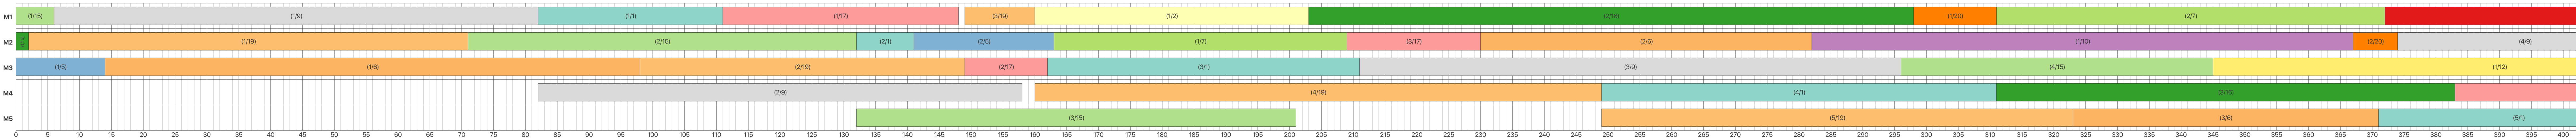
\includegraphics[height=40pt]{figures/solution_pso_instance_3_1_scaled}\\[0.15cm]
\hspace{0.90909pt}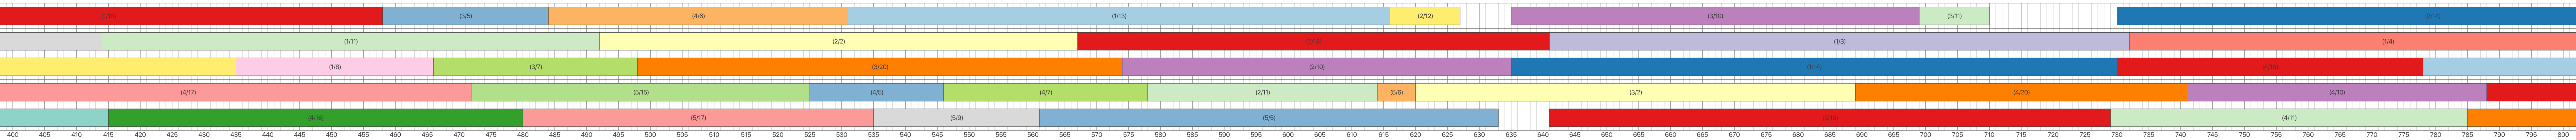
\includegraphics[height=40pt]{figures/solution_pso_instance_3_2_scaled}\\[0.15cm]
\hspace{0.90909pt}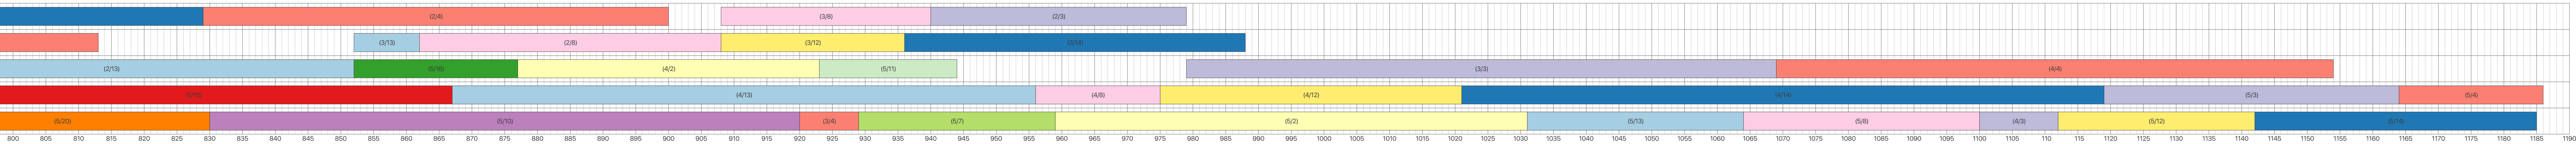
\includegraphics[height=40pt]{figures/solution_pso_instance_3_3_scaled}\\
\multicolumn{1}{c}{\textit{Figure 1: \acf{PSO} solution with makespan 1186 for problem~3 using parameters specified in Table~1.}}\\[1.2cm]
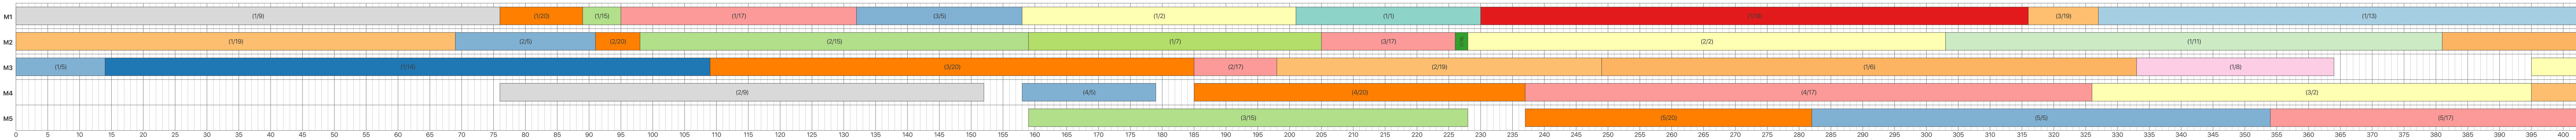
\includegraphics[height=40pt]{figures/solution_aco_instance_3_1_scaled}\\[0.15cm]
\hspace{0.90909pt}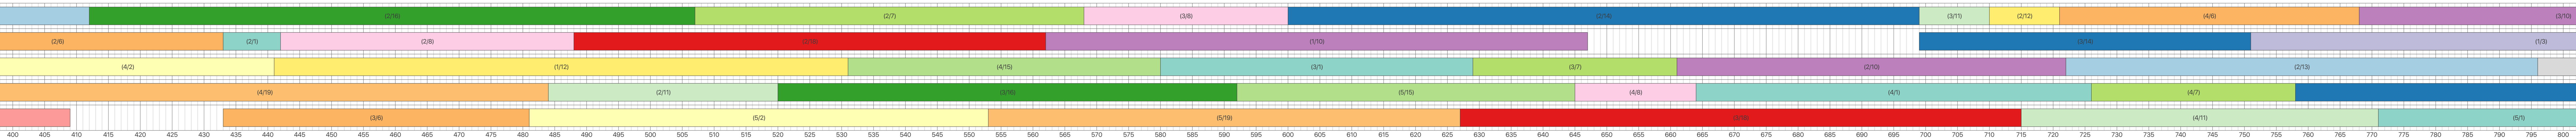
\includegraphics[height=40pt]{figures/solution_aco_instance_3_2_scaled}\\[0.15cm]
\hspace{0.90909pt}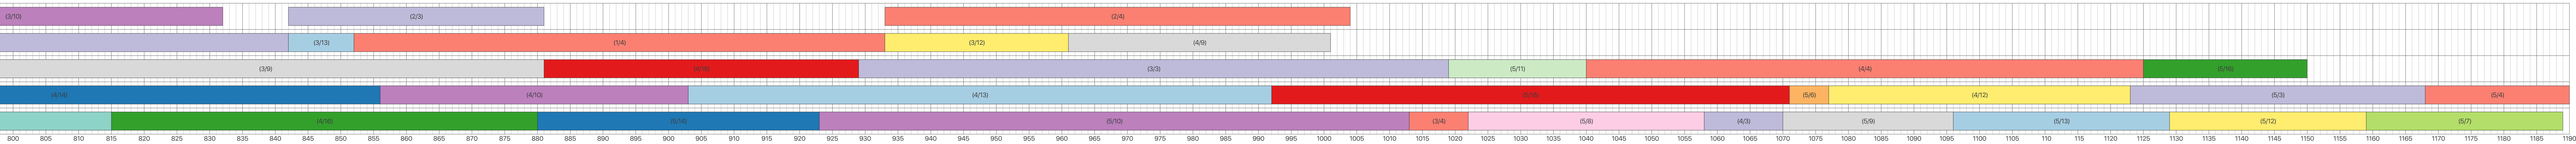
\includegraphics[height=40pt]{figures/solution_aco_instance_3_3_scaled}\\
\multicolumn{1}{c}{\textit{Figure 2: \acf{ACO} solution with makespan 1190 for problem~3 using parameters specified in Table~1.}}\\[1.2cm]
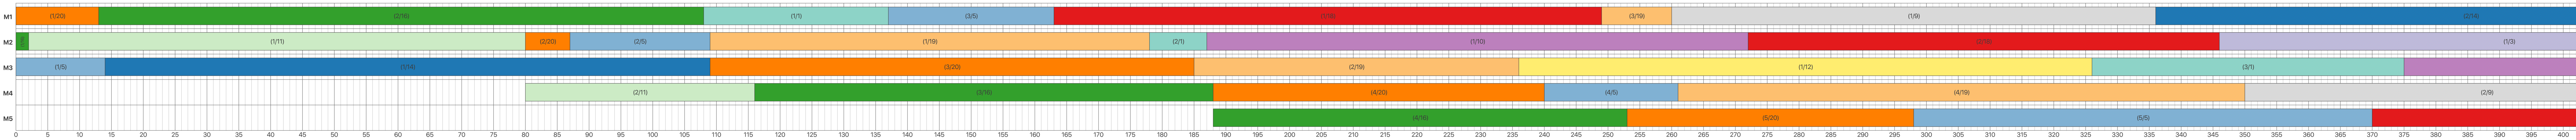
\includegraphics[height=40pt]{figures/solution_ba_instance_3_1_scaled}\\[0.15cm]
\hspace{0.90909pt}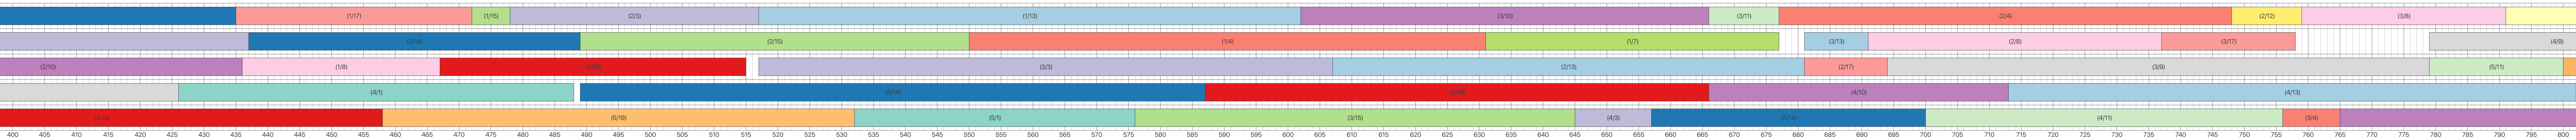
\includegraphics[height=40pt]{figures/solution_ba_instance_3_2_scaled}\\[0.15cm]
\hspace{0.90909pt}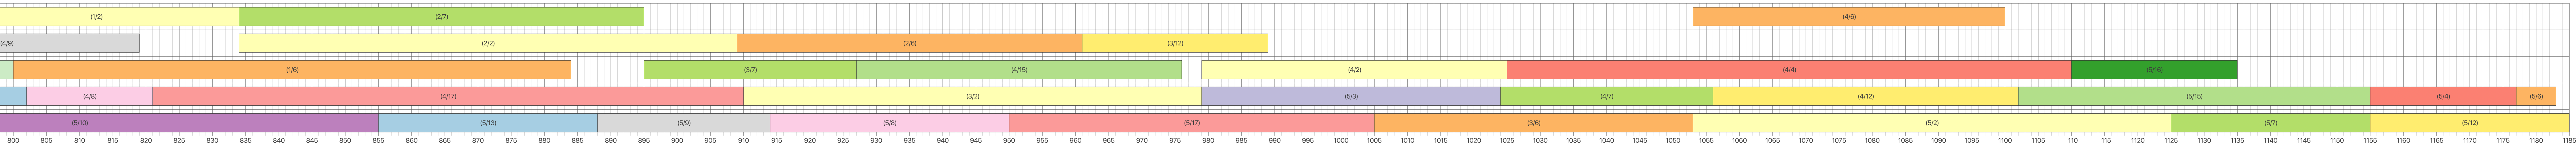
\includegraphics[height=40pt]{figures/solution_ba_instance_3_3_scaled}\\
\multicolumn{1}{c}{\textit{Figure 3: \acf{BA} solution with makespan 1185 for problem~3 using parameters specified in Table~1.}}\\
\end{tabular}
\end{table}
}

\end{landscape}

\end{document}
